\documentclass[11pt]{article}
\usepackage{theme}
\usepackage{shortcuts}
\usepackage{subcaption}
\usepackage{hyperref}
\usepackage[
style=ieee,
]
{biblatex}
\addbibresource{ref.bib}

% Document parameters
% Document title
\title{Mini-Project (ML for Time Series) - MVA 2023/2024}
\author{
Mathis Reymond \email{mathis.reymond74@gmail.com} \\ % student 1
Inès Vati \email{ines.vati@eleves.enpc.fr} % student 2
}

\begin{document}
\maketitle

% \paragraph{What is expected for these mini-projects?}
% The goal of the exercise is to read (and understand) a research article, implement it (or find an implementation), test it on real data and comment on the results obtained.
% Depending on the articles, the task will not always be the same: some articles are more theoretical or complex, others are in the direct line of the course, etc... It is therefore important to balance the exercise according to the article. For example, if you have reused an existing implementation, it is obvious that you will have to develop in a more detailed way the analysis of the results, the influence of the parameters etc... Do not hesitate to contact us by email if you wish to be guided.

% \paragraph{The report}
%  The report must be at most FIVE pages and use this template (excluding references). If needed, additional images and tables can be put in Appendix, but must be discussed in the main document. The report must contain a precise description of the work done, a description of the method, and the results of your tests. Please do not include source code! The report must clearly show the elements that you have done yourself and those that you have reused only, as well as the distribution of tasks within the team (see detailed plan below.)
 
%  \paragraph{The source code}
% In addition to this report, you will have to send us a Python notebook allowing to launch the code and to test it on data. For the data, you can find it on standard sites like Kaggle, or the site https://timeseriesclassification.com/ which contains a lot of signals!


% \paragraph{The oral presentations}
% They will last 10 minutes followed by 5 minutes of questions. The plan of the defense is the same as the one of the report: presentation of the work done, description of the method and analysis of the results.


% \paragraph{Deadlines}
% Two sessions will be available :
% \begin{itemize}
%  \item \textbf{Session 1}
%  \begin{itemize}
%   \item Deadline for report: December 18th (23:59)
%   \item Oral presentations: December 20th and 22th (precise times TBA)
%  \end{itemize}
% \end{itemize}

\section{Introduction and contributions}

% \blue{The Introduction section (indicative length : less than 1 page) should detail the scientific context of the article you chose, as well as the task that you want to solve (especially if you apply it on novel data). \textbf{The last paragraph of the introduction must contain the following information}:
% \begin{itemize}
%     \item Repartition of work between the two students
%     \item Use of available source code or not, percentage of the source code that has been reused, etc.
%     \item Use of existing experiments or new experiments (e.g. test of the influence of parameter that was not conducted in the original article, application of the method on a novel task/data set etc.)
%     \item Improvement on the original method (e.g. new pre/post processing steps, grid search for optimal parameters etc.)
% \end{itemize}}

The article at hand focuses on reviewing the current literature regarding the use of Graph Signal Processing (GSP) methods applied to brain graphs obtained from functional imaging techniques. Within this framework, graph representations illustrate brain regions as nodes and depict connections—be they functional or structural—as edges. This approach, viewing the brain through graphs, holds significance in connectomics and the broader field of network neuroscience. It facilitates the correlation between structural neural connections and the functional connectivity, even extending to behavioral observations.

Authors introduce a Fourier paradigm adapted to graph, including a Graph Fourier Transform (GFT) and graph filters. It allows the decomposition of brain signals based on spatial variability relative to the structure of the brain network. Additionally, they introduce signal surrogate generation, notably to assess significance of their results. They lead two experiments. In the first one, subjects perform a classic Navon switching task : they visualize big symbols made of smaller symbols (as big cross made of small circles). Depending on the colour of the small symbols, participants are asked to report either the shape of small or big symbols. Naturally, the response time is increased when the task switch, which allows defining what's called a switch cost. Using GSP tools, authors have shown that having isolated brain regions highly activated is positively correlated with high switch cost.

Authors provide no code. We wrote our own code for the experiments we conducted. Inès focused on graph surrogates and performed the experiment described in \ref{excursion_results}. Mathis performed on the experiment described in \ref{subsec:classification_results}. We state an equal contribution for the rest of the work carried out. Our code is available on \href{https://github.com/InesVATI/TimeSeries-GraphSignalProcessing}{GitHub}.

Along with qualitative remarks, our contribution lies in the three experiments we conducted. As neither code nor data used in the paper were available, we found another dataset, BOLD5000 \cite{chang_bold5000_2019}, on which we performed experiments using the tools introduced in the article.


\section{Method}

% \blue{The Method section (indicative length : 1 to 2 pages) should describe the mathematical aspects of the method in a summarized manner. Only the main steps that are useful for understanding should be highlighted. If relevant, some details on implementation can be provided (but only marginally).}

We consider a weighted graph $\G = (\V, S)$ where $\V$ is the set of $N$ vertices associated with specific brain regions and $S\in\RR^{N\times N}$ is a matrix connectivity representation (usually the adjacency matrix or Laplacian). We also consider a graph signal $X\in\RR^{N\times T}$ where $T$ is the length of the time series. 

\subsection{Graph Fourier Transform}

In order to define a Fourier transform on $\G$, one must diagonalize this $S$ and express it in the form
\begin{align}
    S = V\Lambda V^{-1}
\end{align}
where $\Lambda$ is a diagonal matrix containing the eigenvalues of $S$, and $V$ is a matrix of associated eigenvectors. This allows the definition, given a signal $x$ on $\G$, of the graph Fourier transform of $x$ on $\G$ as
\begin{equation}
    \widetilde{x} := V^Tx \label{eq:GFT}
\end{equation}
Please refer to the appendix \ref{app:fourier_t} for the computations that draw parallels with the discrete Fourier transform on temporal data.

\subsection{Graph filtering}
In the context of graph signal processing, filters are commonly defined within the spectral domain. Let $h$ be a transfer function, and we denote $H$ as the diagonal matrix where $H_{ii} = h(\lambda_i)$, and $\lambda_i$ denotes the eigenvalues of $S$. The filtered signal $Y_h\in \RR^{N\times T}$ is defined as follows 
\begin{equation}
    Y_h := VHV^TX
\end{equation}
In this formulation, filtering is applied independently to each time sample $x[t]$. However, unlike traditional time-domain filtering, graph filtering leverages the graph structure to smooth the signal across its edges rather than along the time axis. This distinction becomes obvious when visualizing the impact of graph filtering on a signal. Figure \ref{fig:visu_filt_signal} illustrates the differences in the same signal, either filtered with a low-pass filter or a high-pass filter. Colour values on the low-pass filtered signal exhibit greater homogeneity across nodes than on the high-pass filter one. 

\subsection{Generation of graph surrogate signals}

Statistical testing is crucial when it comes to make inferences about the properties of signals. For example, we may want to test whether the observed signal is significantly different from a random signal. 
Phase-randomization in the temporal Fourier domain \cite{theiler_testing_1992} offers to preserve the spectral properties of the time series while randomizing the signal. It consists in generating surrogate data from an original time series by randomizing the phases of the original time series while keeping the magnitudes of the Fourier components unchanged. The surrogate signal is given by $Y = XF^H\phi_{time}F$, where $\phi_{time}$ contains random phase factors, $F$ and $F^T$ indicate the temporal Fourier Transform and Inverse Fourier Transform, respectively. \\
We can extend this procedure to the graph framework : $Y=V\phi_{graph}V^TX$ where $\phi_{graph}$ is a diagonal matrix containing random phase factors. $\phi_{graph}$ can be defined by random sign flips of the graph spectral coefficients. An explanatory scheme is provided in Figure \ref{surr_scheme}. 
% The obtained surrogate signal $Y$ is a random signal with the same power spectrum as $X$ but with randomized phase and the non-stationary spatial effects are destroyed.


In \cite{huang_graph_2018}, one of the objectives is to discern significant signal excursions, which are distinct moments in time when brain activity enters a regime of strong alignment or liberality. \\
In the context of the authors' study, alignment and liberality are concepts used to characterize different aspects of functional brain activity. Alignment is associated with regions of the brain that activate simultaneously. On the other hand, liberality pertains to areas that exhibit high signal variability, suggesting a more diverse and dynamic pattern of activity. Alignment is computed using a low-pass filter on the graph because low-pass filters allow the preservation of lower-frequency components while attenuating higher-frequency variations. Liberality, conversely, is computed using a high-pass filter on the graph that emphasizes higher-frequency variations. The authors employed the following procedure to compute excursions in those different regimes :
\begin{enumerate}
    \item capture alignment and liberality with low-pass and high-pass filters on the original signal
    \item generate 1,000 null surrogate signals for each filtered signal, as performed in \cite{pirondini_spectral_2016}
    \item employ the generated null data to threshold the filtered signals at a $\alpha$-level of 5\%
\end{enumerate}


\section{Data}
% \textit{The Data section (indicative length : 1 page) should provide a deep analysis of the data used for the experiment. In particular, we are interested here in your capacity to provide relevant and thoughtful feedbacks on the data and to demonstrate that you master some "data diagnosis" tools that have been dealt with in the lectures/tutorials.}

\subsection{BOLD5000 dataset}

We used the BOLD5000 database \cite{chang_bold5000_2019} in our experiments. It is a large-scale fMRI dataset that captures brain scans from four patients as they view over 5,000 images. The dataset covers a wide range of visual features, categories, and semantics, and can be used to test various hypotheses and models related to visual cognition. \\
fMRI produces 4D images, relying on the principle that localized neural activity induces changes in metabolism and blood flow.
% \red{, resulting in fluctuations in the concentrations of oxyhemoglobin\footnote{Oxyhaemoglobin are the red cells in the blood that carry oxygen} and deoxyhemoglobin\footnote{the same red cells after they have delivered the oxygen}. Oxyhaemoglobin and deoxyhaemoglobin have different magnetic properties\footnote{Oxyhemoglobin is diamagnetic, while deoxyhemoglobin is paramagnetic}, and they affect the local magnetic field in different ways.}
To record cerebral activity during functional sessions, the scanner is tuned to detect this "Blood Oxygen Level Dependent" (BOLD) signal. 
Brain activity is measured in sessions that span several minutes, during which participants are presented with a variety of images. Simultaneously, participants engage in a valence judgment task for each stimulus, expressing their preference using the descriptors "like", "neutral", and "dislike", which are encoded with labels 1, 2, and 3.\\
As the mapping between descriptors and labels was not provided, we inferred it ourselves.

\subsection{Time series extraction and diagnosis}

For each region of interests (ROIs) in the dataset, we extracted the time series, which represents the temporal activity in the brain. We used Nilearn -a Python library that provides tools for neuroimaging data analysis- to extract the signals.
Signal extraction is usually achieved by averaging the fMRI time series across the voxels in a region \cite{varoquaux_learning_2013}. 

In this study, time series were $z$-scored, \ie shifted to zero mean and scaled to unit variance. We also took into account the confounds in the extraction, as there were provided in the database. Confounds are variables that can affect the brain signal and are not of interest in the study. They can include head motion, physiological noise, and scanner artefacts. In order to extract clean signals from brain regions, it is important to remove the effects of confounds from the data. 
% This is done by regressing out the confounds from the data before extracting the signals. 

The time series obtained from the regions of interest (ROIs) do not appear to be noisy, as shown in Figure \ref{fig:plot_TS}. One can assume that signal are weak stationary as their mean and autocorrelation does not appear to vary over time. The spectrogram plotted in figure \ref{spectrogram_TS} shows that their spectral properties does noes not change over time. They all exhibit the same variability and mean as they were z-scored. Their values range between $-2.5$ and $2.5$, except for some regions that have extreme values or outliers (see Fig \ref{fig:boxplot_TS}). They seem to have the same spectral properties except for the retrosplenial complex (RSC) region in left and right hemisphere which has a more chaotic spectrum. Those results are shown in figure \ref{fig:spectral_TS}.

\subsection{Brain Graph Construction}

In order to represent the strength of axonal connection (structural connectivity), authors of \cite{huang_graph_2018} defined $A_{ij}$ as a simple count of the number of streamlines - \ie estimated individual fibers that connect the regions - using diffusion spectrum imaging. However, since we did not have access to this information, we defined the adjacency matrix $\A$ in another manner. In our setting, it corresponds to the connectivity matrix between brain regions (functional connectivity). Indeed, the extracted signals can be used to compute a correlation matrix between the regions \cite{varoquaux_learning_2013}. It is a common metric for computing the edges between the nodes, and is depicted in figure \ref{fig:connectivity}.




\section{Results}
% \blue{The Result section (indicative length : 1 to 2 pages) should display numerical simulations on real data. If you re-used some existing implementations, it is expected that this section develops new experiments that were not present in the original article. Results should be discussed not only based on quantative scores but also on qualitative aspects. In particular (especially if your article focuses on black box methods), please provide some feedbacks whether the method was adapted to the data or not and whether the hypothesis behind the approach you used were validated or not.}

\subsection{Extract excursions in alignment and liberality regimes}
\label{excursion_results}

In this section, we investigate the following questions : (i) In our setting with only 10 regions, can we exhibit regions with frequent moments of strong alignment and liberality ? (ii) Does the choice of low-pass or high-pass filter influence the percentage of significant excursions ? (iii) What do we obtain if we apply the conventional phase Fourier randomization ?

Mirroring the approach of the authors \cite{huang_graph_2018}, we propose a non-parametric, model-free statistical test for identifying unexpected fluctuations in time series magnitude over time. 
We compute the average of the (temporal) 95\% percentile on the surrogate signals, as illustrated in Figure \ref{fig:statistic_surr}. The obtained value is used to threshold the "true" time series. The time points that exceed this threshold are said to be significant excursions.
The protocol is repeated for all the $20$ runs and statistical results are plotted in Figure \ref{fig:result_excursions_filters}. \\ 
The authors  chose the 12\% smallest and largest eigenvalues for the alignment and liberality filters, respectively. It comes down to almost 2 eigenvalues for our graph. 
We implement the equivalent version of the filters and two other continuous filters that are displayed in Figure \ref{fig:filt}. The continuous low-pass filter is defined by $h_{low,\ continuous}(x) = \frac{1}{1 + \tau x}$ with $\tau = 3$ and the continuous high-pass filter is given by $ h_{high,\ continuous}(x) = \frac{2}{1 + \exp(-\tau (x - r) ) }$ with $\tau = 1$ and $r = 5$.
% \begin{align}
%     h_{low,\ continuous}(x) &= \frac{1}{1 + \tau x} \label{filt_low_cont} \\
%     h_{high,\ continuous}(x) &= \frac{2}{1 + \exp(-\tau (x - r) ) } \label{filt_high_cont}
% \end{align}

The study by Huang et \textit{al.} \cite{huang_graph_2018} focused on $87$ brain regions, in contrast to our dataset with only $10$ regions. Consequently, it is unsurprising that we do not replicate their reported percentage of excursions. Our findings, depicted in Figure \ref{fig:result_excursions_filters}, reveal two key observations: (i) the inability to identify regions with a high percentage of excursions, attributed to the limited number of studied regions; and (ii) the similarity in results between continuous and non-continuous low-pass filters. However, for high-pass filters, certain regions, such as the left hemisphere lateral occipital cortex (LHLOC) and the retrosplenial complex (RSC), do not have the same percentage of excursions and the same variability. This discrepancy may be attributed to the high-pass continuous filter accepting more eigenvalues than its non-continuous counterpart,  as illustrated in Figure \ref{fig:filt}. Notably, the majority of eigenvalues surpass $3$. Thus, the continuous low-pass filter select a sufficient number of low eigenvalues compare to the non-continuous low-pass filter, which is not replicated by the continuous high-pass filter.\\
Moreover, (iii) Figure \ref{fig:result_Fourier_excursions} indicates that performing a statistical test with the conventional randomization do not exhibit differences between the brain regions. This outcome is anticipated, given that the phase randomization matrix $\phi$ is uniformly applied to the nodes of the graph in the same manner. However, the article \cite{huang_graph_2018} reported that alignment excursions persist when employing conventional randomization.
% The persistence of alignment excursions under this randomization method suggests that there are spatial dynamics in the brain's functional activity that are non-random and may be associated with specific functional connections among brain regions. 
We can argue that our inability to replicate these results stems from the limited availability of labelled brain regions in our dataset.

\subsection{Utilizing Neural Correlates to Predict Subjective Experience of Visual Stimuli}\label{subsec:classification_results}

In this experiment, we aim to employ GSP tools to predict the subjective preference of pictures. Specifically, using the BOLD5000 brain images, our objective is to predict categorical labels : 1, 2, or 3. In order to avoid subtleties caused by inter-subject studies, we confine this experiment to data acquired solely during the initial 6 runs of the first session of subject CSI1.

We compute 6 matrices sized (10, 194) corresponding to the activation levels of the 10 brain regions across the 194 time points. This process enables the computation of a connectivity matrix for each of the 6 runs, where connectivity is derived as the average connectivity across the 194 time points. To create a unified representation, we compute the average connectivity matrix from the set of 6 connectivity matrices, which allows defining a brain graph based on this final averaged matrix. We perform diagonalization of the Laplacian matrix associated to this graph, enabling for graph Fourier transform. Given the graph's 10 vertices, for each of the $6\times194$ time points, we compute the graph Fourier transform of the activation across the 10 brain regions projected on the graph. This process yields $6\times194$ samples, each comprising 10 features: the Fourier coefficients.

Using the Sklearn, we train both a simple Multi-Layer Perceptron and a Gradient Boosting Tree. Training involves 80\% of the vectors made of the squared Fourier coefficients. Then, we evaluate the models' performance on the remaining 20\% of the data. Regrettably, we do not observe any improvements in balanced accuracy as compared to random classification. However, as this approach breaks down the temporal continuity by considering individual vectors without accounting for the fact that the complete response pattern for each image spans 4 to 5 time points, it was expected to obtain poor results.

That's why, ultimately, we tried to perform dictionary learning, with the aim to extract specific patterns for each appreciation. Unfortunately, as the patterns we are looking for are 4 to 5 time points long, dictionary learning is not very suited to extract them. 

\subsection{Subjective Experience Prediction with K-Nearest Neighbors and Distance Time Warping}

We refer to a "sub-sequence" as the segment within the time series when the patient is observing a single image. Those sub-sequences last approximately $10$ seconds and have a temporal length of 4 to 6 time points. \\ 
In this section, our objective is to classify these sub-sequences using a k-Nearest Neighbors (K-NN) algorithm. Let's index the sub-sequences with $I$ and for any $i\in I$, let's denote the temporal lengths of the sub-sequence $i$ with $T_i$. Consider $X_i\in\RR^{N\times T_i}$ and $X_j\in\RR^{N\times T_j}$ as two sub-sequences. They may have different temporal lengths. Recall that $N$ is the number of brain regions. We define the distance between $X$ and $Y$ as
$$
d(X_i, X_j) = \frac{1}{N}\sum_{n=1}^N DTW(X_i[n], X_j[n])
$$
where $DTW$ is the Distance Time Warping (DTW) measure. \\
Using Scikit-learn, we implemented a cross-validation to compare results across various number of neighbors. The balanced accuracies are depicted in Figure \ref{knn_5_fold}. The only model surpassing the chance level is the one with $k=3$ neighbors, displaying a median accuracy of $40$\%. However, the variability remains substantial. This may be explained by the relatively short length of the sub-sequences. Furthermore, caution is advised when independently comparing sub-sequences from different runs.

\printbibliography

\appendix
\appendixpage % ajoute par defaut le titre "Appendices" au dessus de la première annexe
\section{Parallel with Discrete Fourier Transform}
\label{app:fourier_t}

Pour développer l'intuition, et voir plus clairement le parallèle avec la transformée de Fourier discrète, il peut être intéressant de se demander si un graphe permet de retrouver l'interprétation habituelle de la transformée de Fourier discrète d'un signal temporel. Les graphes cycliques permettent cela. En effet, soit un signal $x$ sur le graphe cycle à $N$ sommets $C_N$. La matrice laplacienne $L_N$ de ce graphe s'écrit, pour $N=6$ 
\[ L_6 := 
\begin{bmatrix}
2 & -1 & 0 & 0 & 0 & -1 \\
-1 & 2 & -1 & 0 & 0 & 0 \\
0 & -1 & 2 & -1 & 0 & 0 \\
0 & 0 & -1 & 2 & -1 & 0 \\
0 & 0 & 0 & -1 & 2 & -1 \\
-1 & 0 & 0 & 0 & -1 & 2 \\
\end{bmatrix}
\]
En notant
\[J_N :=
\begin{bmatrix}
0 & 1 & 0 & \dots & 0 \\
0 & 0 & 1 & \dots & 0 \\
\vdots  &     &     & \ddots & \vdots  \\
0 & & &        & 1 \\
1 & 0 & 0 & \dots  & 0
\end{bmatrix}
\]
on observe que 
\begin{align}
    L_N = 2I_N - J_N - J_N^{N-1}
\end{align}
Or les valeurs propres de $J$ sont les racines $N$-ièmes de l'unité $\omega^0,...,\omega^{N-1}$ où $\omega := e^{\frac{2i\pi}{N}}$ et pour tout $k\in [\![0,N-1]\!]$, \[X_k := \begin{bmatrix} 1 \\\omega^k \\ \omega^{2k}\\ \vdots\\ \omega^{(N-1)k}\end{bmatrix}\]
est vecteur propre de $J$ associé à la valeur propre $\omega^k$.
Cela permet donc, en notant $W$ la matrice de transformée de Fourier discète
\[ W :=
\begin{bmatrix}
1&1&1&1&\cdots &1 \\
1&\omega&\omega^2&\omega^3&\cdots&\omega^{N-1} \\
1&\omega^2&\omega^4&\omega^6&\cdots&\omega^{2(N-1)}\\ 1&\omega^3&\omega^6&\omega^9&\cdots&\omega^{3(N-1)}\\
\vdots&\vdots&\vdots&\vdots&\ddots&\vdots\\
1&\omega^{N-1}&\omega^{2(N-1)}&\omega^{3(N-1)}&\cdots&\omega^{(N-1)(N-1)}
\end{bmatrix}
\]
d'écrire
\begin{align}
    L_N = W(2I_N -\Omega-\Omega^{N-1})W^{-1}
\end{align}
où $\Omega := Diag(w^0,...,w^{N-1})$\\
Ainsi, les valeurs propres de $L_N$ sont les $\lambda_k = 2 - \omega^k - \omega^{-k}$ pour $k \in [\![0,N-1]\!]$.\\
En utilisant la définition de la transformée de Fourier sur les graphes \ref{eq:GFT}, on explicite le $k$-ième coefficient de Fourier
\begin{align}
    \Tilde{x}_k &= W_k^*x\\
    &= \overline{W_k}x\\
    &= \sum_{n=0}^{N-1}x_n\omega^{-nk} \\
    &= \sum_{n=0}^{N-1}x_n e^{-2i\pi n\frac{k}{N}}
\end{align}
On retrouve la définition de la transformée de Fourier discrète.

\begin{figure}[h]
  \centering
  \begin{subfigure}{0.35\linewidth}
    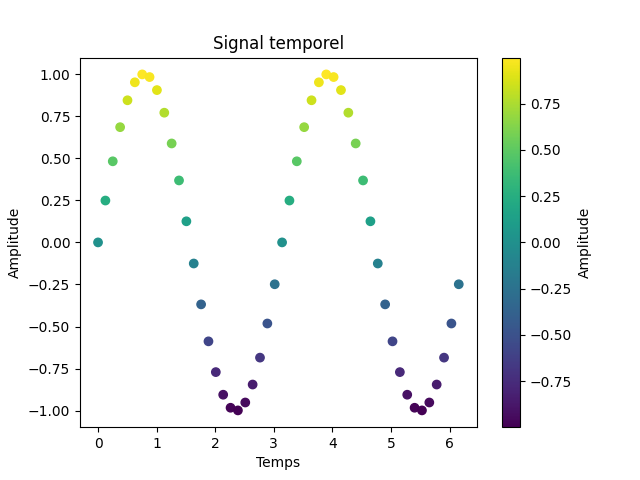
\includegraphics[width=6.5cm]{img/temporal_signal.png}
    \caption{Représentation temporelle d'un signal echantillonné}
    \label{fig:DANN_1}
  \end{subfigure}
  \hspace{1.5cm}
  \begin{subfigure}{0.35\linewidth}
    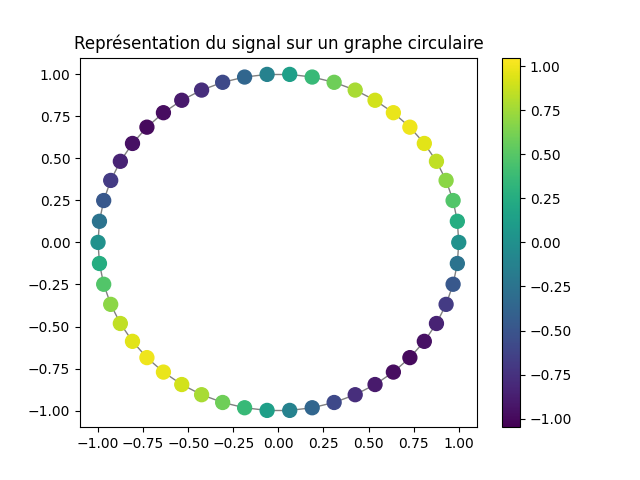
\includegraphics[width=6.5cm]{img/graph_signal.png}
    \caption{Représentation du même signal sur un graphe circulaire}
    \label{fig:DANN_2}
  \end{subfigure}
  \caption{Deux représentations d'un signal échantillonné dont on calcule la transformée de Fourier par les deux définitions dont on dispose : la transformée de Fourier discrète, et la transformée de Fourier d'un graphe}
  \label{fig:DANN
}
\end{figure}

\section{Data visualization}

\subsection{MRI Image}
\begin{figure}
    \centering
    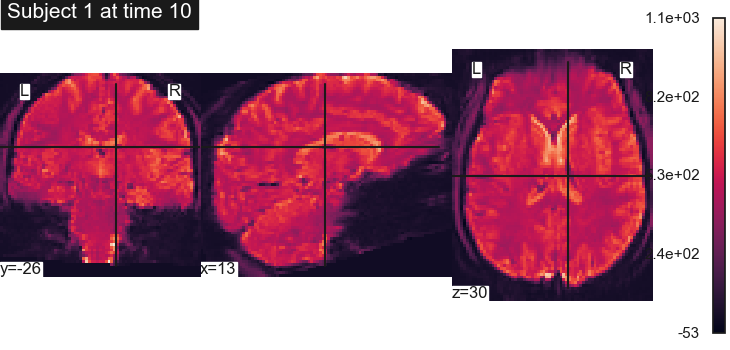
\includegraphics[width=\textwidth]{img/example_fmri.png}
    \caption{Example of a 3D MRI plotted for the first patient}
    \label{fig:ex_mri}
\end{figure}

\subsection{Time series diagnosis}
\begin{figure}
    \begin{subfigure}{\textwidth}
        \centering
        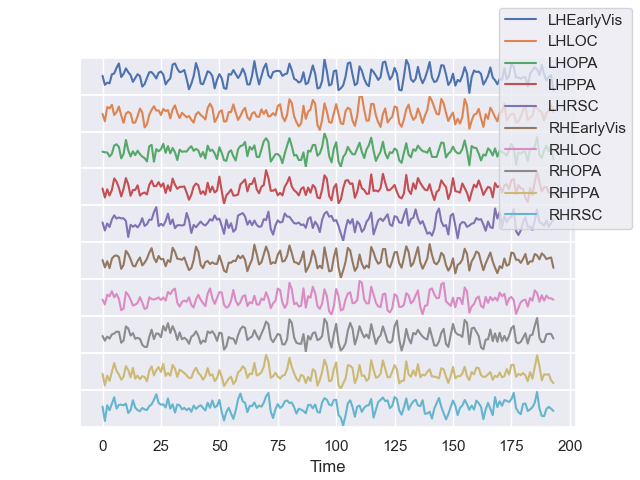
\includegraphics[height=.4\textheight]{img/plot_time_series.png}
        \caption{Time series in each region of interests}
        \label{fig:plot_TS}
    \end{subfigure}
    \begin{subfigure}{\textwidth}
        \centering
        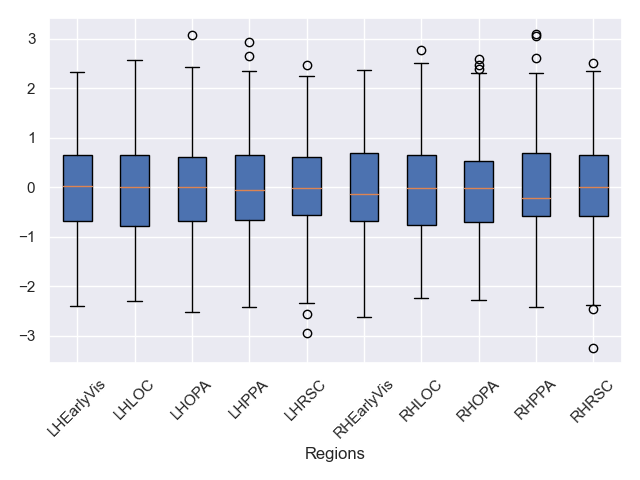
\includegraphics[height=.4\textheight]{img/boxplot_time_series.png}
        \caption{Box plot of the time series}
        \label{fig:boxplot_TS}
    \end{subfigure}
    \caption{Analysis of the extracted time series. There were 10 ROIs: early visual (EarlyVis), lateral occipital cortex (LOC), occipital place area (OPA), parahippocampal place area (PPA), retrosplenial complex (RSC) for the left hemisphere (LH) and right hemisphere (RH).} 
    \label{fig:analysis_TS}
\end{figure}

\begin{figure}
    \centering
    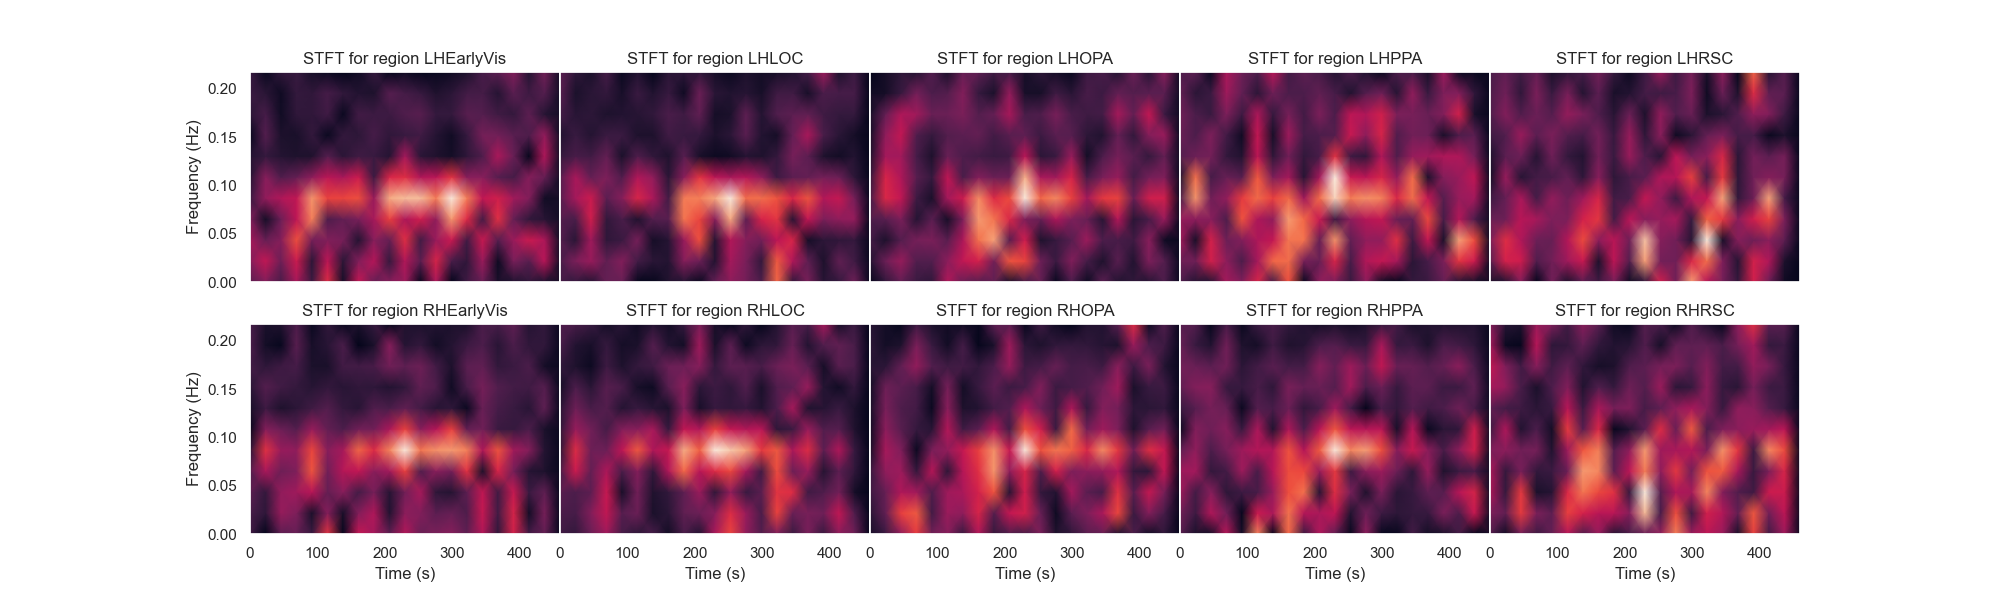
\includegraphics[width=\textwidth, height=0.25\textheight]{img/autocorrelation_TS.png}
    \caption{Autocorrelation analysis across various brain regions. Not all results were plotted to enhance readability.}
    \label{fig:autocorr_TS}
\end{figure}

\begin{figure}
    \centering
    \begin{subfigure}{\textwidth}
        \centering
        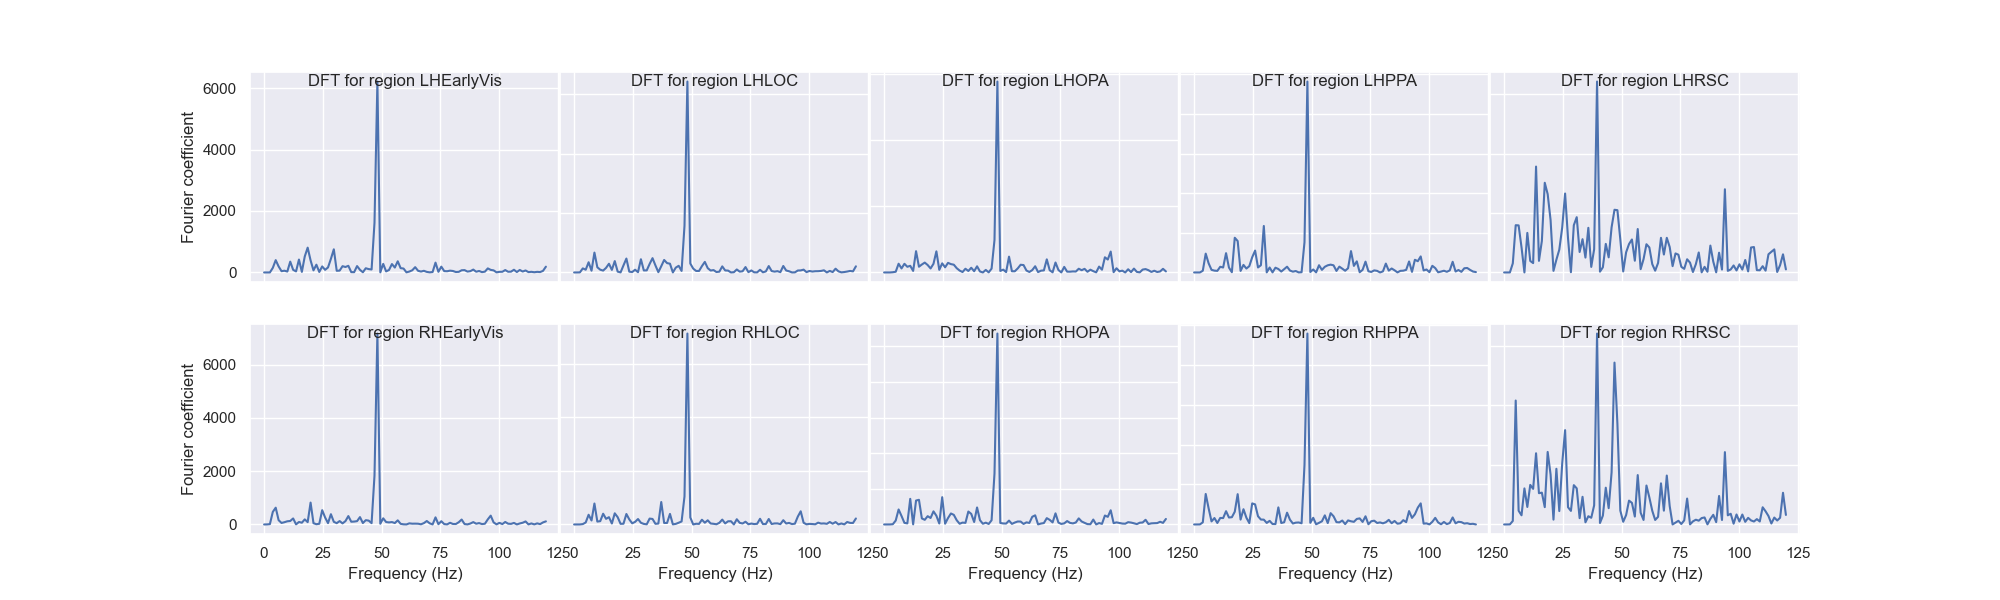
\includegraphics[width=\textwidth, height=0.28\textheight]{img/DFT_TS.png}
        \caption{Discrete Fourier Transform (DFT)}
    \end{subfigure}
    \begin{subfigure}{\textwidth}
        \centering
        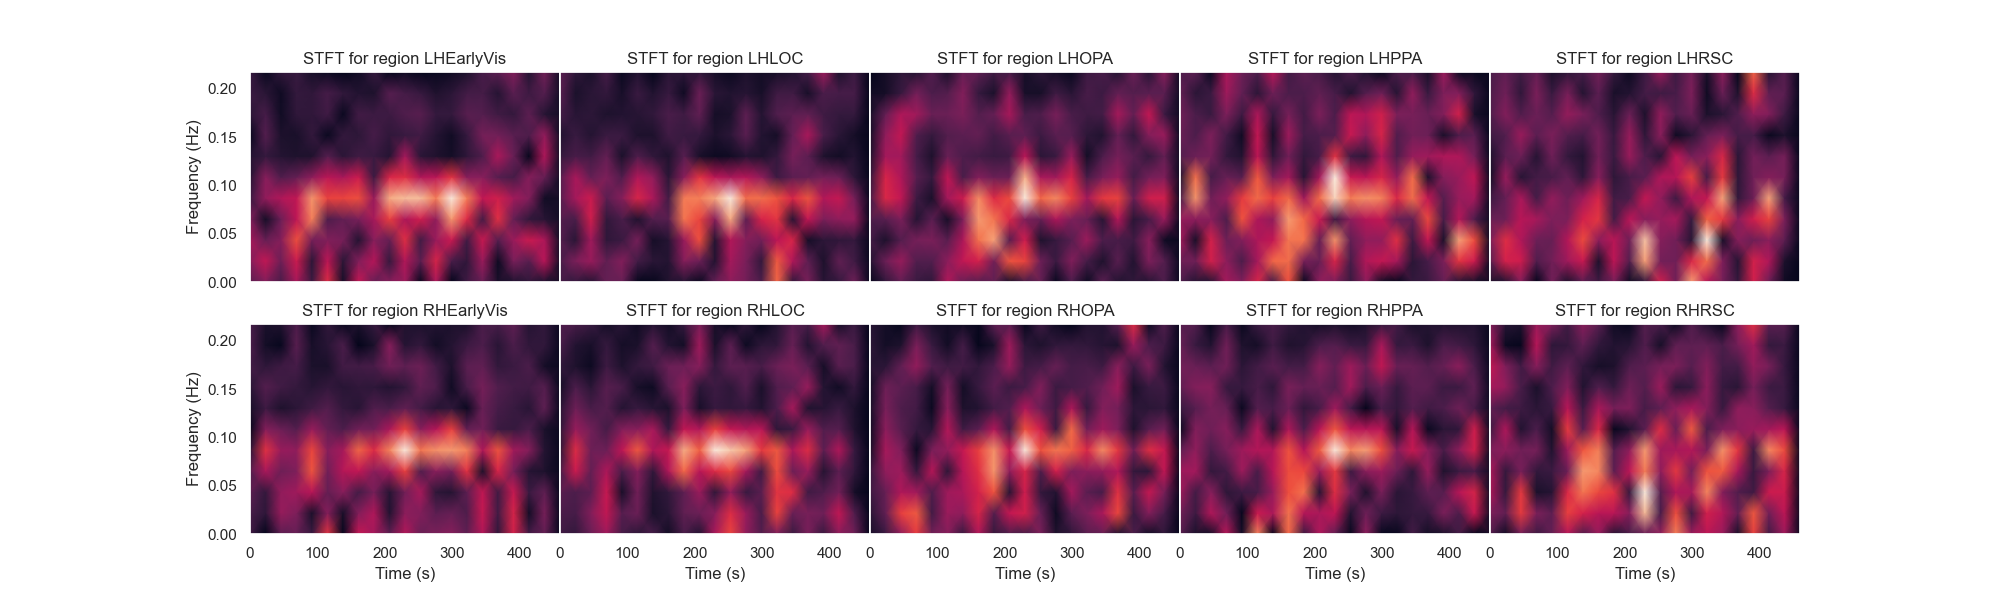
\includegraphics[width=\textwidth, height=0.25\textheight]{img/spectrogram_TS.png}
        \caption{Spectrogram}
        \label{spectrogram_TS}
    \end{subfigure}
    \caption{Spectral analysis of the time series for each brain region. (b) The spectrogram was computed with window length of $20$ and an overlapping of $16$.}
    \label{fig:spectral_TS}
\end{figure}

\section{Graph Construction}

\begin{figure}[H]
\centering
    \begin{subfigure}{\textwidth}
        \centering
        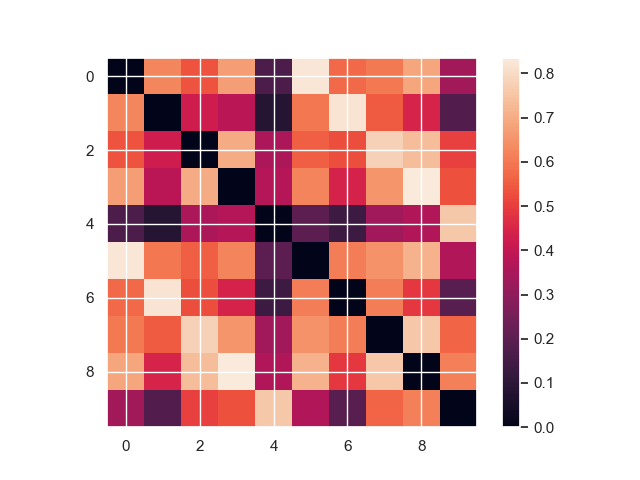
\includegraphics[height=.35\textheight]{img/connectivity_matrix.png}
        \caption{Connectivity matrix}
        \label{fig:connectivity}
    \end{subfigure}
    \begin{subfigure}{\textwidth}
        \centering
        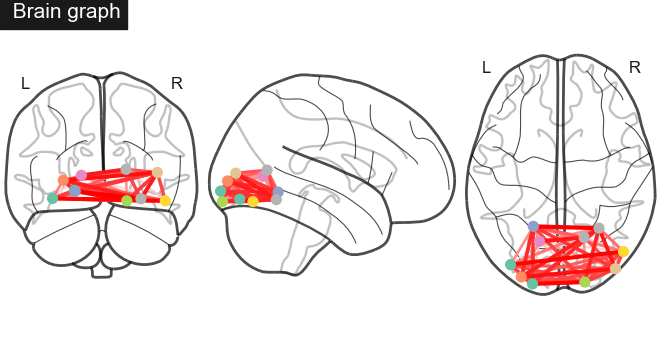
\includegraphics{img/brain_graph.png}
        \caption{Functional-connectome graph}
        \label{ex_graph}
    \end{subfigure}
    \caption{Representation of the brain graph. (a) Connectivity matrix for a given patient, which is also the adjacency matrix $\A$ of the graph $\G$. The entry $A_{i,j}$ of the connectivity matrix is obtained by computing the correlation coefficient between the time series extracted from regions $i$ and $j$. (b) displays the corresponding \textit{connectome}. This representation offers a unique insight into the patient’s
neural architecture, highlighting the potential correlates of cognitive processes}
    \label{fig:brain_graph}
\end{figure}

% \begin{figure}
%     \centering
%     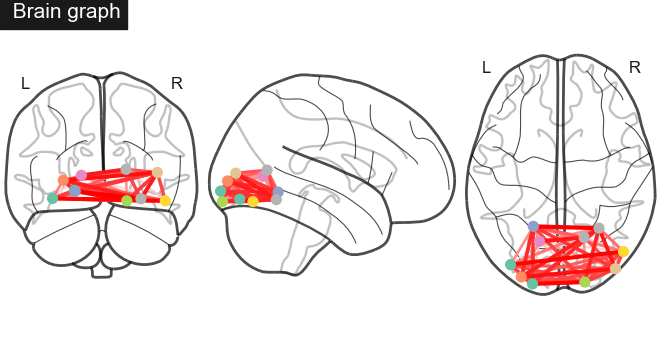
\includegraphics{img/brain_graph.png}
%     \caption{Caption}
%     \label{fig:enter-label}
% \end{figure}

\section{Filters}

\begin{figure}
    \centering
    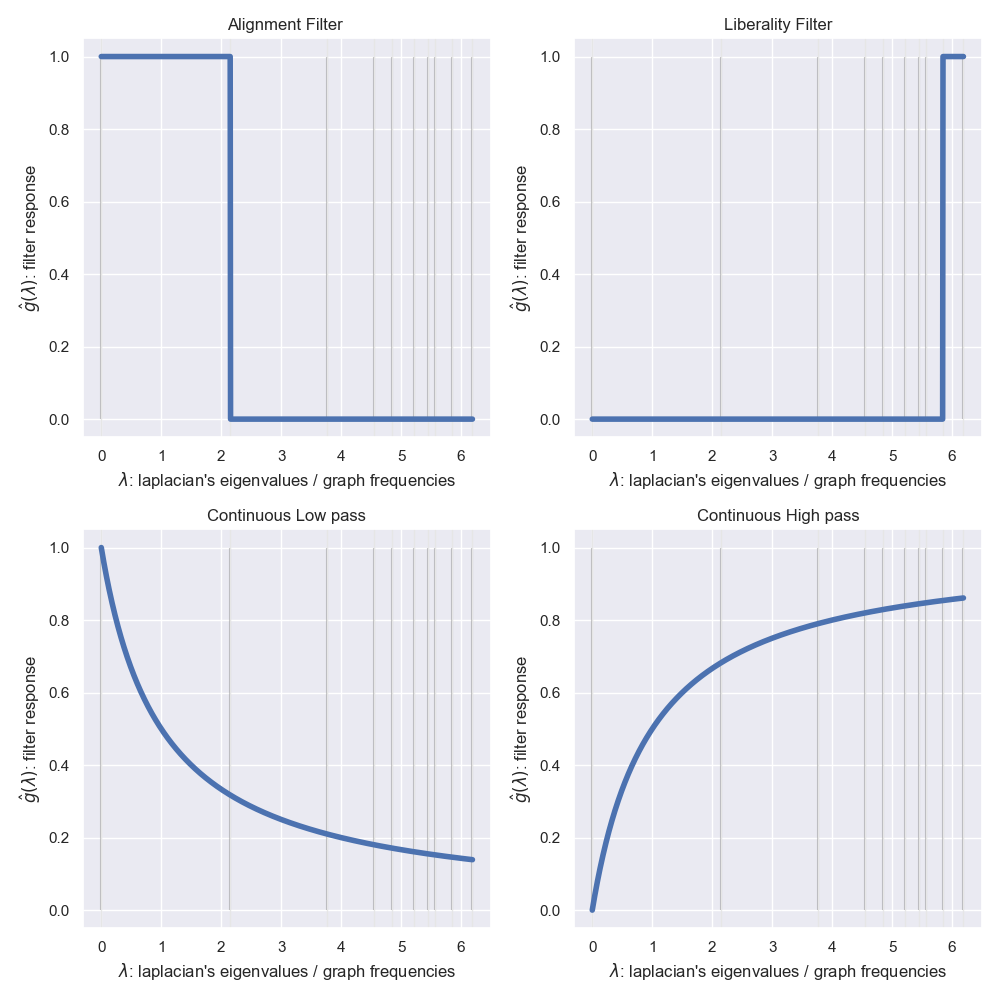
\includegraphics{img/plot_filters.png}
    \caption{Comparison of different filters for graph signal analysis. The \textit{alignment filter} and the \textit{liberality filter} are the low-pass filter and high-pass filter, respectively, employed in the article\cite{huang_graph_2018}. The authors defined their filters by considering the $10$\% lowest and largest eigenvalues, respectively.  In our context, this comes down to filtering approximately 2 eigenvalues.}
    \label{fig:filt}
\end{figure}

\begin{figure}
    \centering
    \begin{subfigure}{\textwidth}
        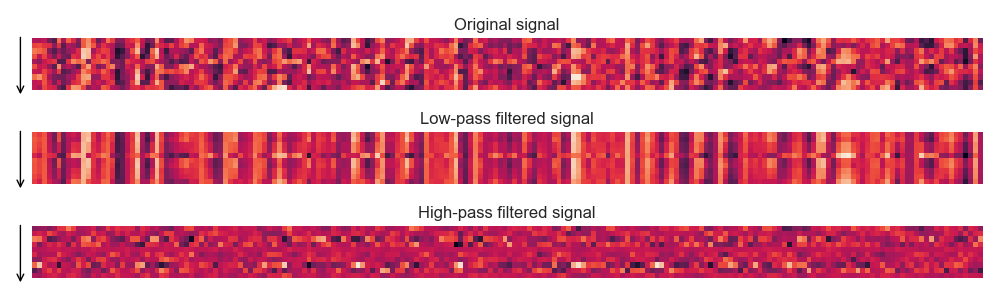
\includegraphics[width=\textwidth]{img/ex_filtered_signal.png}
        \caption{Filtered signal $Y_H$}
    \label{fig/ex_filt_signal}
    \end{subfigure}
    \begin{subfigure}{\textwidth}
        \centering
        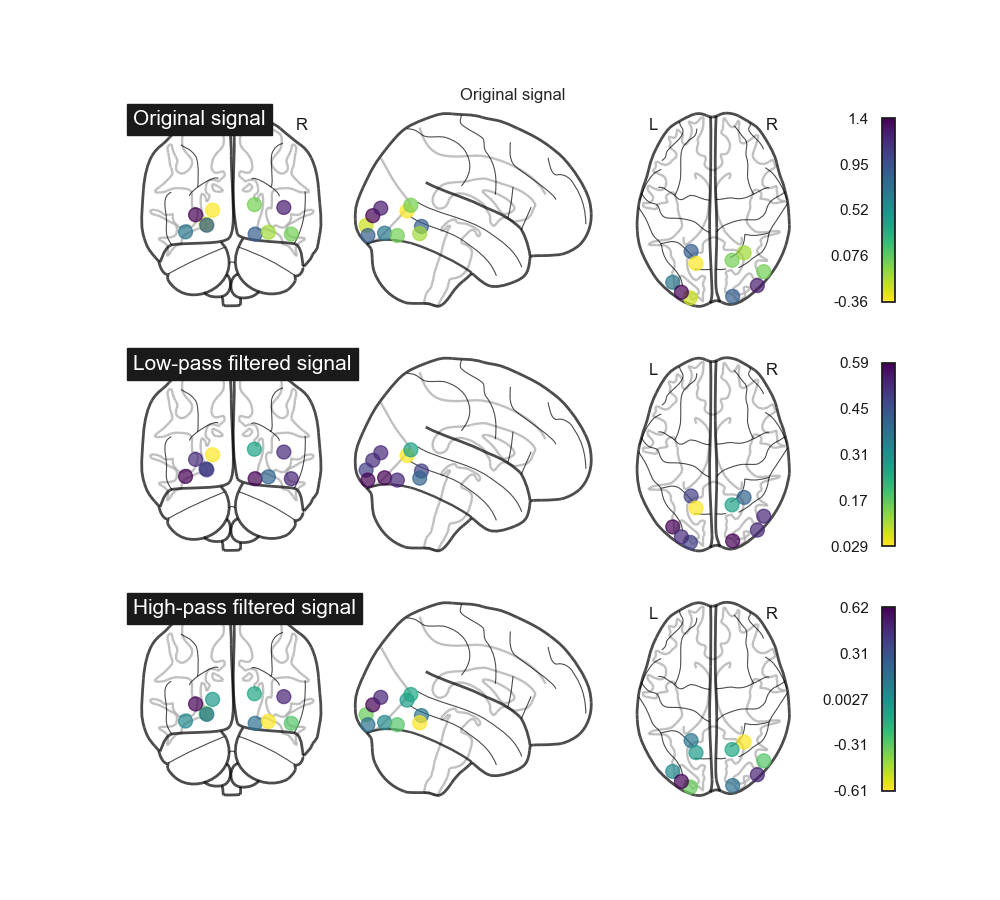
\includegraphics[width=\textwidth]{img/ex_filtered_signal_markers.png}
        \caption{Filtered signal at time $t=0$ in the brain graph.}
        \label{fig:ex_filt_markers}
    \end{subfigure}
    \caption{Visualization of the filtered signals at each time point in (a) and on the graph in (b). (a) The down arrow in $y$-axis indicates the brain regions. The $x$-axis corresponds to the time axis. (b)}
    \label{fig:visu_filt_signal}
\end{figure}

\section{Test statistic}

\begin{figure}
    \centering
    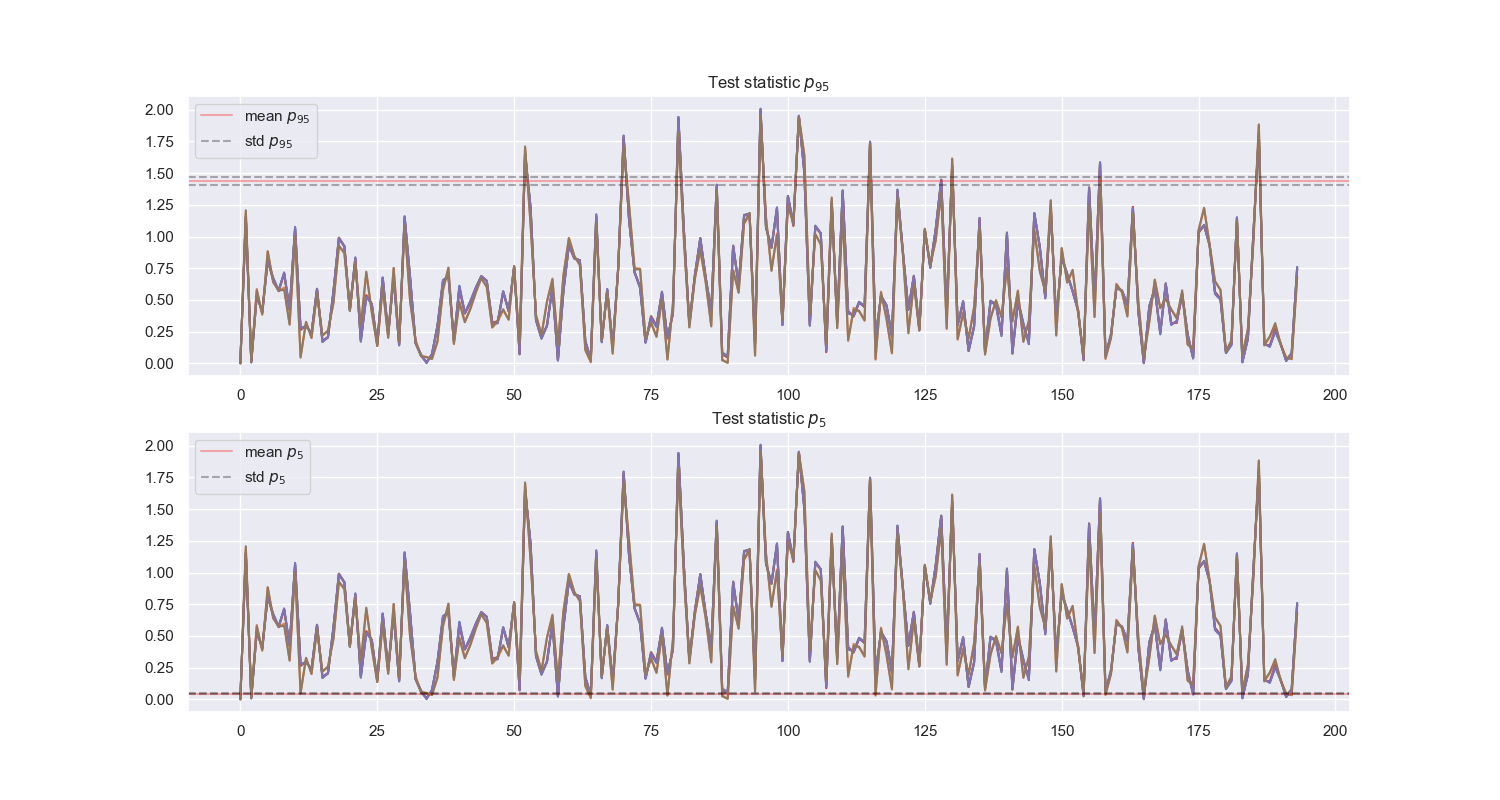
\includegraphics{img/plot_ex_surrogate.png}
    \caption{Threshold computed on the surrogate signals. $p_{95}$ and $p_{5}$ are respectively the average of the 95\% and 5\% (for significant low amplitude) percentile on the surrogate signals.}
    \label{fig:statistic_surr}
\end{figure}

\begin{figure}
    \centering
    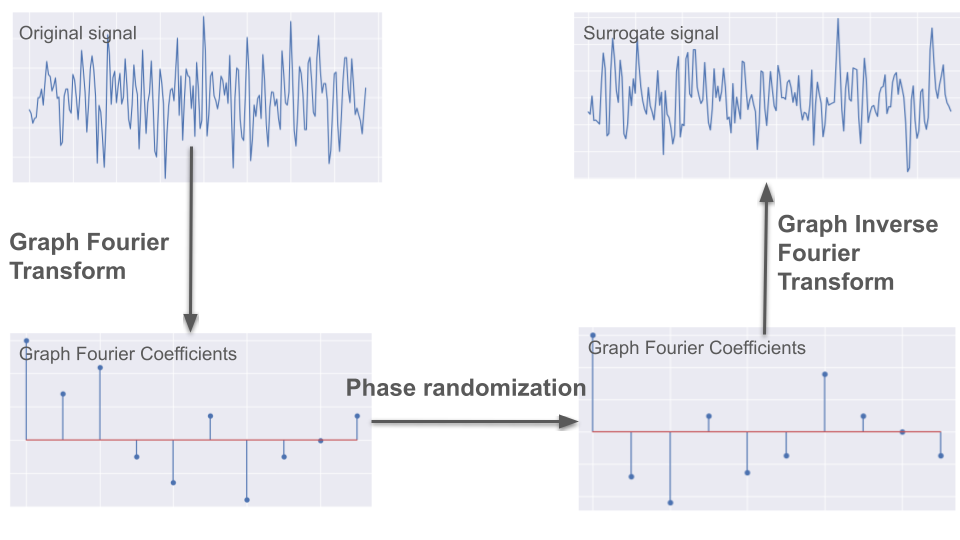
\includegraphics{img/surrogate_scheme.png}
    \caption{Surrogate signal generation scheme.}
    \label{surr_scheme}
\end{figure}

\section{Results on computing excursions}

\begin{figure}
    \centering
    \begin{subfigure}{0.45\textwidth}
        \centering
        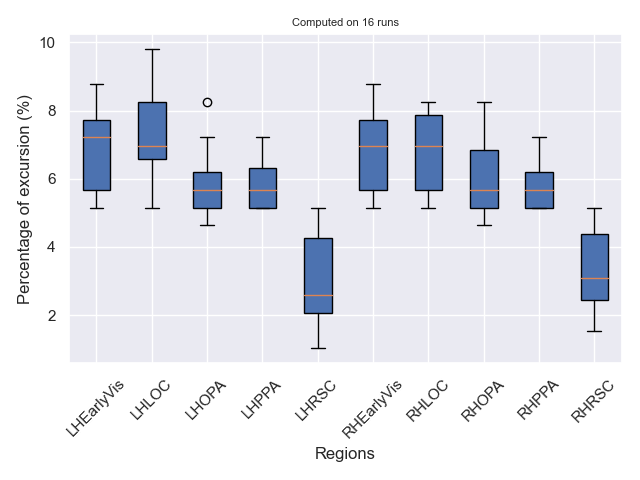
\includegraphics[width=\textwidth]{img/low_non_continuous_filter_graph_randomization.png}
        \caption{Article-inspired low-pass filter}
    \end{subfigure}
    \hfill
    \begin{subfigure}{0.45\textwidth}
        \centering
        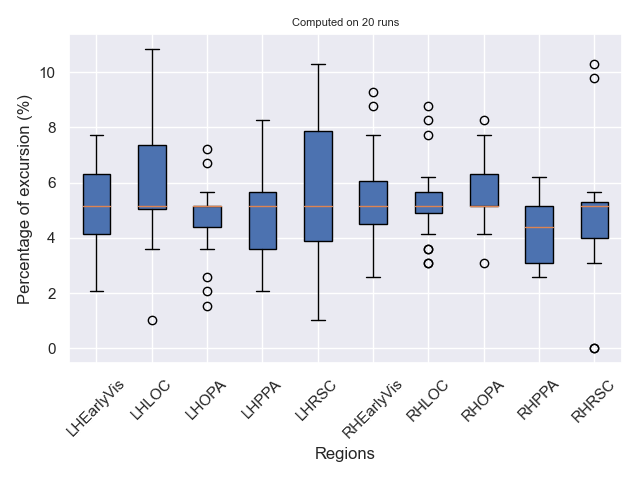
\includegraphics[width=\textwidth]{img/high_non_continuous_filter_graph_randomization.png}
        \caption{Article-inspired high-pass filter}
    \end{subfigure}
    \hfill
    \begin{subfigure}{0.45\textwidth}
        \centering
        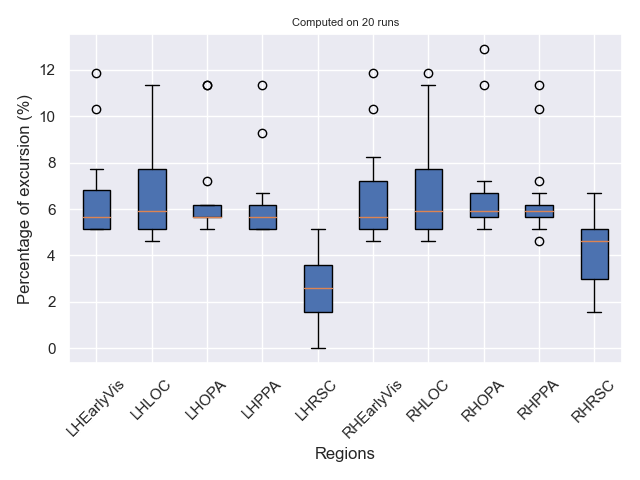
\includegraphics[width=\textwidth]{img/low_continuous_filter_graph_randomization.png}
        \caption{Continuous low-pass filter}
    \end{subfigure}
    \hfill
    \begin{subfigure}{0.45\textwidth}
        \centering
        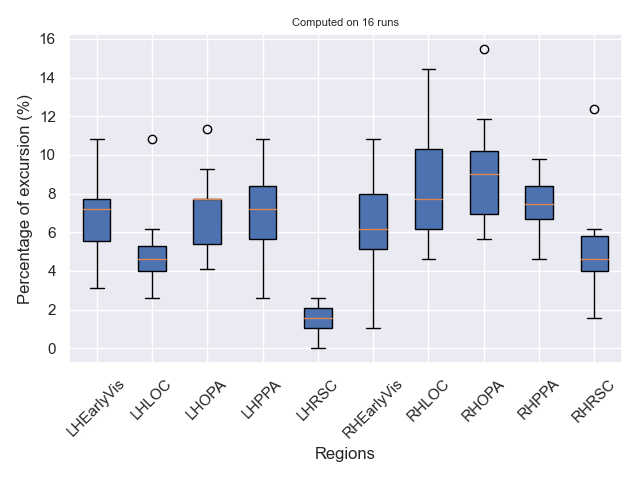
\includegraphics[width=\textwidth]{img/high_continuous_filter_graph_randomization.png}
        \caption{Continuous high-pass filter}
    \end{subfigure}
    \caption{Comparison of different filters for computing excursions in alignment and liberality regimes. The method outlined in section \ref{excursion_results} were repeated on $20$ different fMRI of the same patient. For each run, we generate 1,000 null surrogate graph signal.}
    \label{fig:result_excursions_filters}
\end{figure}

\begin{figure}
    \centering
    \begin{subfigure}{.45\textwidth}
        \centering
        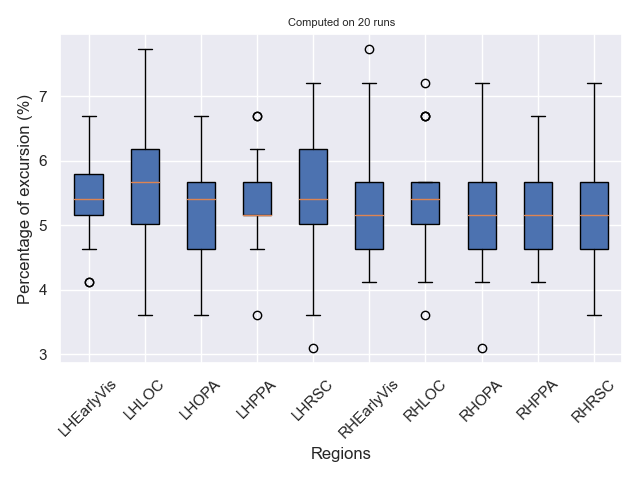
\includegraphics[width=\textwidth]{img/low_continuous_filter_Fourier_randomization.png}
        \caption{Continuous low-pass filter}
    \end{subfigure}
    \hfill
    \begin{subfigure}{.45\textwidth}
        \centering
        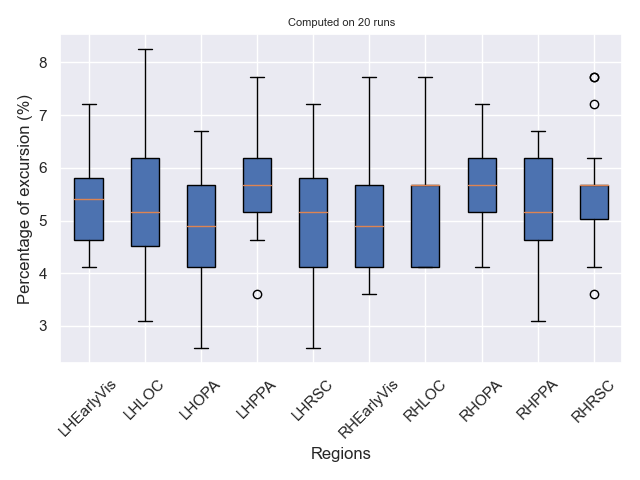
\includegraphics[width=\textwidth]{img/high_continuous_filter_Fourier_randomization.png}
        \caption{Continuous high-pass filter}
    \end{subfigure}
    \caption{Results using the conventional phase Fourier randomization in the temporal domain.}
    \label{fig:result_Fourier_excursions}
\end{figure}
\section{Accuracy of the k-NN with DTW}

\begin{figure}
    \centering
    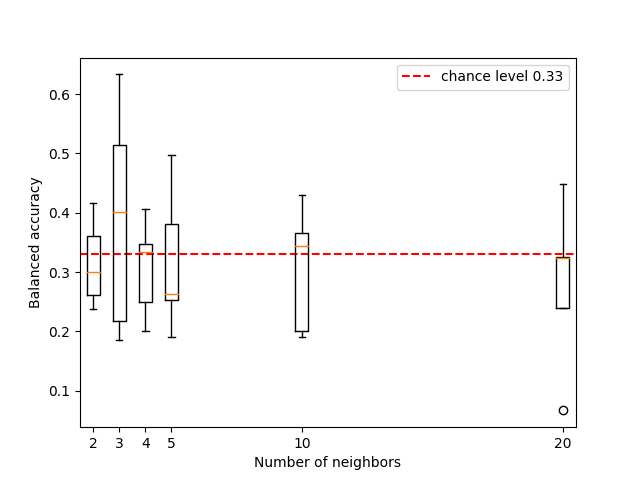
\includegraphics{img/5-fold_knn_scores.png}
    \caption{5-fold cross-validation of the model combining DTW and k-neighbours classifier.}
    \label{knn_5_fold}
\end{figure}

\end{document}
